 \chapter{Metodologia}
 
Este capítulo apresenta a estrutura geral do sistema, que se divide em duas partes. A primeira consiste no \textit{backend} desenvolvido em Python com o objetivo de reconhecer as etiquetas utilizando técnicas de \textit{Machine Learning}. A segunda parte compreende o sistema web, desenvolvida em Node.JS, responsável pela visualização e gerenciamento do sistema através de relatórios e telas.

A validação do projeto será feita através de um sistema que seja capaz de identificar números localizados em etiquetas em uma única imagem.

%------------------------------------------------

\section{Visão geral do sistema} \label{sec:funcionamento}

Esta seção descreve as características operacionais do sistema, assim como os resultados esperados. O fluxo geral do sistema é apresentado visualizado na Figura \ref{fig:arqgeral}.

\begin{figure}[htbp]
	\centering
	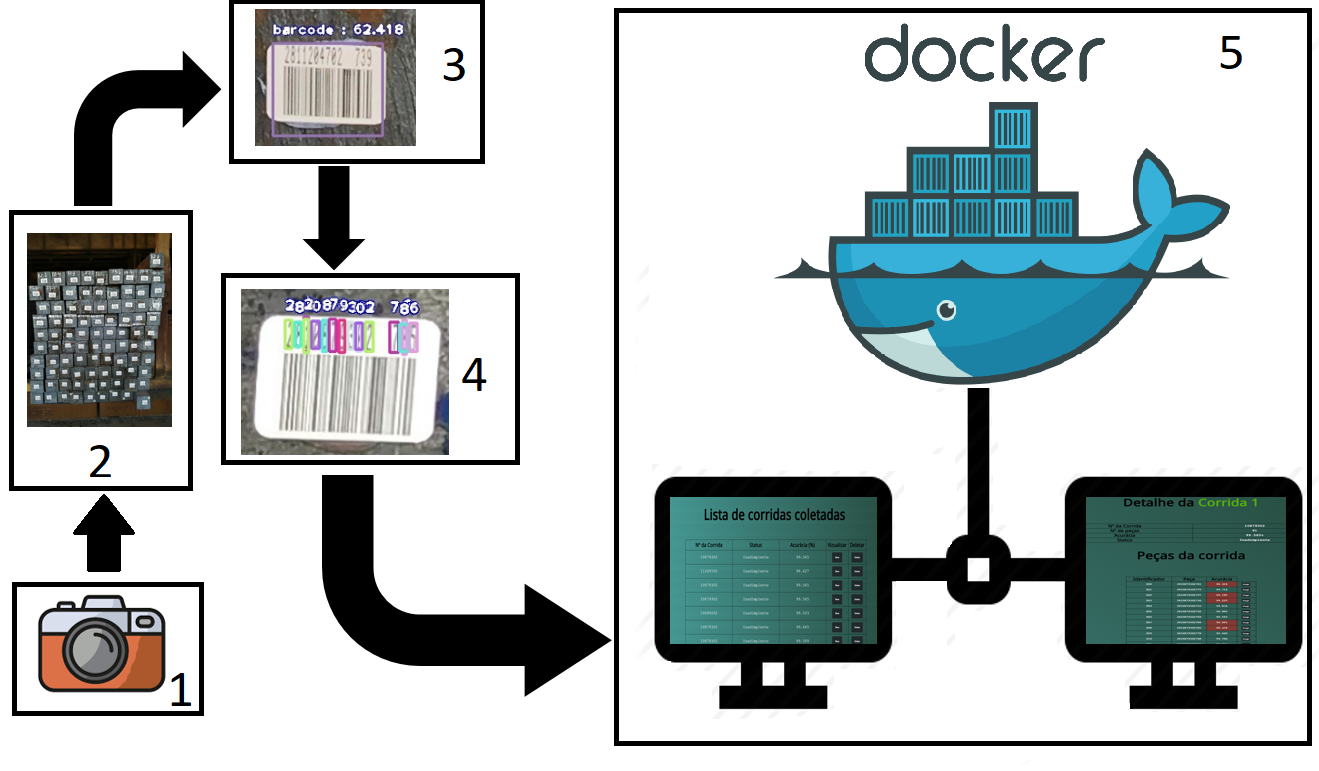
\includegraphics[width=1\linewidth]{capitulos/FluxoDoProjeto.png}
	\caption{Arquitetura geral do projeto.}
	\begin{tabular}{r@{: }l r@{: }l}
    1 & Câmera Fotográfica & 4 & Identificação de números \\
    2& Foto das peças da corrida & 5 & Sistema WEB \\
    3 & Identificação dos códigos de  barra
    \end{tabular}
	\label{fig:arqgeral}
\end{figure}

O projeto será organizado será realizado em etapas sequenciais. Será iniciado ao se fotografar as peças de uma corrida no setor de despacho utilizando uma câmera comum. 

A fotografia iniciará automaticamente o fluxo do sistema e, a partir dela, terá início o reconhecimento da imagem. Os códigos de barras localizados nas etiquetas de cada tarugo são detectados, recortados automaticamente e salvos separadamente em imagens contendo apenas uma etiqueta. Em seguida, os números são identificados.

A corrida é salva em um banco de dados e exibida através de telas para que o usuário possa validá-las.

A comunicação entre os dois sistemas, de detecção e web, acontece através do resultado da saída do sistema de detecção, que são os números localizados acima do código de barras de cada etiqueta. Posteriormente estes números são  gravados em um arquivo JSON para que o sistema web possa receber e mostrar através das telas. 

%------------------------------------------------

\section{Backend em Python} \label{sec:backend}

Para realizar o experimento, é necessário treinar um modelo de rede neural que seja capaz de reconhecer código de barras e algarismos numéricos. Para isso, são efetuadas três etapas. Primeiro é coletado o maior número possível de imagens dos códigos de barras. Em seguida, é gerado um \textit{dataset} com as características dessas imagens juntamente com a classe em que pertence. Então, é possível realizar a configuração e treinamento da rede neural. Por fim é calculada a acurácia, mediante imagens de teste, do modelo que obteve a melhor performance no treinamento.

A linguagem de programação Python para implementação do sistema de detecção foi prioritariamente escolhida devido à grande comunidade existente, ao grande número de bibliotecas de análise de dados disponíveis e ao fato da ferramenta Google Colab utilizá-lo, permitindo o alto processamento dos dados, o que não seria possível em um computador de baixa performance.

%------------------------------------------------

\subsubsection*{Python}

Linguagem interpretada é uma linguagem de programação em que o código fonte é executado por um \textit{software} chamado interpretador, que em seguida é executado pelo sistema operacional ou processador

Python é uma linguagem de programação interpretada de alto nível, ou seja, com um nível de abstração relativamente elevado e de uso geral. 

Suporta vários paradigmas de programação, incluindo programação estruturada (principalmente processual), orientada a objetos e funcional.

Sua abordagem orientada a objetos tem a finalidade de ajudar os programadores a escrever código para projetos de pequena e grande escala.

Os interpretadores de Python estão disponíveis para diversos sistemas operacionais. Uma organização sem fins lucrativos, a Python Software Foundation, gerencia e direciona recursos para o desenvolvimento do Python. \cite{van2007python}

%------------------------------------------------

\subsection{Preparação do dataset}

Em \textit{websites} públicos é possível encontrar diversos \textit{datasets} \textit{open source}. Utiliza-se um repositório aberto com imagens de código de barras. Esse repositório possui 500 imagens e foi disponibilizado pelo laboratório \textit{Applied Recognition Technology Laboratory}. O grande volume de imagens compreende especificamente diferentes tipos de códigos de barras.\cite{Arte-Lab}

\begin{figure}[htbp]
	\centering
	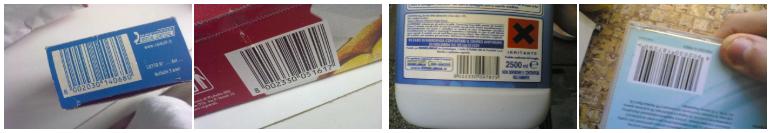
\includegraphics[width=1\linewidth]{figuras/MachineLearning/barcodes.png}
	\caption{Dataset dos código de barras}
	\label{fig:datasetBarcode}
\end{figure}

Para o treinamento de um modelo de rede neural é desejável que se tenha o maior número possível de imagens no \textit{dataset} para um treinamento mais preciso. Além da grande quantidade já obtida com o repositório, utiliza-se o método de \textit{Data Augmentation} para aumentar a quantidade de dados para o treinamento.  

%------------------------------------------------

\subsubsection*{\textit{Data Augmentation}}\label{sec:dataAugm}

\textit{Data Augmentation} é o processo de aumentar a quantidade e diversidade de dados de forma sintética. A partir de uma imagem, é possível gerar mais imagens similares através de métodos como girar um ângulo arbitrário, embaçar a imagem, alterar o brilho, e/ou ofuscando-a.

Mesmo quando os dados são de qualidade inferior (\textit{e.g.} em imagens com baixa nitidez) os algoritmos de ML podem ter bom desempenho, desde que dados úteis possam ser extraídos pelo modelo do conjunto de dados original. Por exemplo, os modelos de conversão de texto em fala e em texto melhoraram devido ao lançamento de um corpus\footnote{Um corpus pode ser entendido como uma coleção de porções de texto selecionadas de acordo com um conjunto de critérios para representar, tanto quanto possível, uma determinada língua \cite{sinclair2005corpus}} de trilhões de palavras pelo Google \cite{halevy2009unreasonable}. Esse resultado ocorre apesar dos dados serem coletados de páginas da web não filtradas e conter muitos erros.\cite{dataAug}

O Código \ref{cod:dataaug} abaixo mostra o momento em que é definido o tipo de ação que será feita em cada foto, como rotacionar em um ângulo aleatório, inserir ruído na imagem e girar horizontalmente. O método também possibilita escolher a quantidade de imagens que será gerada. Neste caso, 1000 imagens.

\begin{lstlisting}[caption=Exemplo de código do método \textit{data augmentation}, label=cod:dataaug][H]
 num_files_desired = 1000
 available_transformations = {
                                'rotate': random_rotation,
                                'noise': random_noise,
                                'horizontal_flip': horizontal_flip
                             }
\end{lstlisting}

%------------------------------------------------

\subsection{Anotações das imagens}

Após criar o \textit{dataset}, as anotações das imagens geradas são feitas. É criado um arquivo que contém as posições dos \textit{pixels} da \textit{Bounding Box} que engloba o objeto na imagem. Um dos formatos mais conhecidos é o Pascal VOC. O formato VOC do Pascal utiliza arquivos XML para armazenar as informações sobre os objetos anotados nas imagens. Para que seja possível gerar tais arquivos mais facilmente, foi utilizado o software LabelImg.

%------------------------------------------------

\subsubsection*{\textit{Bounding Box}}

A \textit{Bounding Box}(bbox) (Figura \ref{fig:boundingBox}) é um dos métodos de anotação de imagem mais populares usados em \textit{Machine Learning} e em \textit{Deep Learning}.

As bbox são caixas retangulares que podem ser determinadas pelo recorte da imagem baseado nas coordenadas das extremidades. Comop exemplo, as bbox do cachorro e do gato da Figura \ref{fig:boundingBox} são definidas com base nas informações de coordenadas da imagem superior. \cite{allDeep}

\begin{figure}[H]
		\centering
		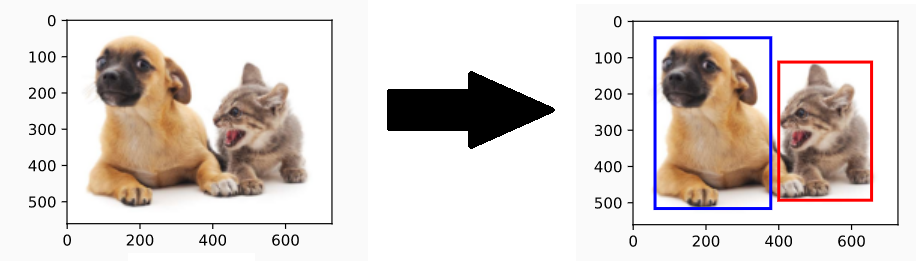
\includegraphics[scale=0.6]{figuras/MachineLearning/catDog.png}
		\caption{Execução de \textit{Bounding Boxes}.}
		\legend{Fonte: \cite{133Ob9905723:online})}
		\label{fig:boundingBox}
\end{figure}

O código \ref{cod:bbox} refere-se à posição das \textit{Bounding Boxes} do cachorro e do gato na imagem, respectivamente.

\begin{lstlisting}[caption=Posições de X e Y nas \textit{Bounding Boxes}, label=cod:bbox]
         dog_bbox, cat_bbox = [60, 45, 378, 516], [400, 112, 655, 493]
\end{lstlisting}

%------------------------------------------------

\subsubsection*{LabelImg}\label{sub:LabelImg}

O LabelImg (Figura \ref{fig:labelimg}) é uma ferramenta \textit{open source} de anotação de imagem gráfica escrita em Python. As anotações são salvas em arquivos XML no formato PASCAL VOC (Código \ref{cod:XML}), o formato usado pelo ImageNet. Além disso, também suporta o formato YOLO, utilizado no projeto. \cite{labelimg}

O software em questão permite que as bbox sejam circuladas englobando o objeto de interesse nas imagens e criando automaticamente um arquivo XML com todas as especificações necessárias.

Utiliza-se o LabelImg para formar o \textit{dataset} que é usado para testar o desempenho do algoritmo. Obter dados suficientes para realizar o experimento costuma ser uma dificuldade visto que é necessário um grande volume de informação. Os \textit{datasets open source} ajudam a resolver esta questão ao disponibilizar diversos conjuntos de dados. Alguns \textit{datasets} comumente usados na visão computacional são os seguintes:

\begin{figure}[H]
	\centering
	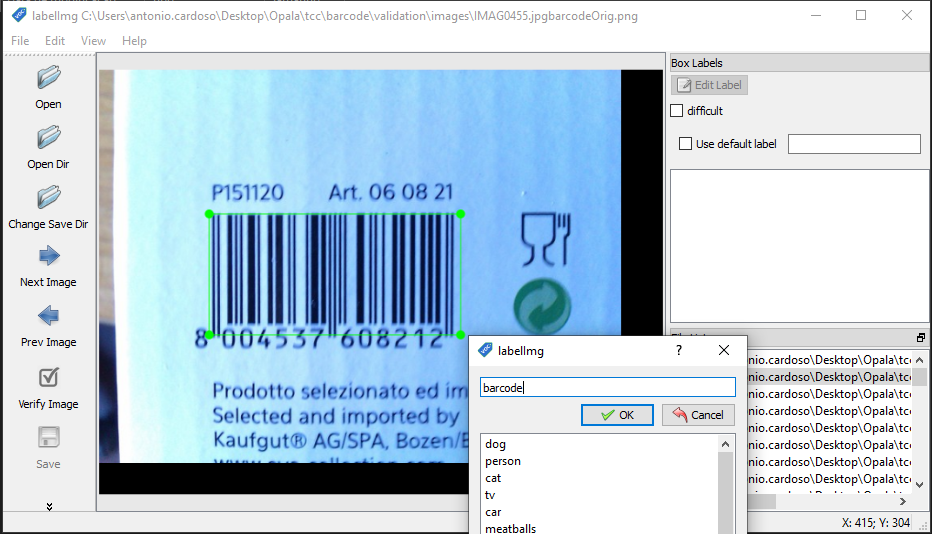
\includegraphics[width=0.9\linewidth]{figuras/MachineLearning/labelimg.png}
	\caption{Procedimento de anotações das \textit{bounding boxes}}
	\label{fig:labelimg}
\end{figure}

\begin{lstlisting}[caption=Arquivo XML gerado pelo LabelImg, label=cod:XML]
<annotation>
	<folder>images</folder>
	<filename>05102009081.jpgbarcodeOrig.png</filename>
	<path>C:\Users\antonio.cardoso\Desktop\tcc\barcode\train\images\05102009081.jpgbarcodeOrig.png</path>
	<source>
		<database>Unknown</database>
	</source>
	<size>
		<width>640</width>
		<height>480</height>
		<depth>3</depth>
	</size>
	<segmented>0</segmented>
	<object>
		<name>barcode</name>
		<pose>Unspecified</pose>
		<truncated>0</truncated>
		<difficult>0</difficult>
		<bndbox>
			<xmin>105</xmin>
			<ymin>63</ymin>
			<xmax>536</xmax>
			<ymax>454</ymax>
		</bndbox>
	</object>
</annotation>
\end{lstlisting}

O ImageNet \textit{dataset} \cite{deng2009imagenet} possui mais de 14 milhões de imagens, cobrindo mais de 20.000 categorias. Existem mais de um milhão de imagens com anotações explícitas de classe e de locais de objetos na imagem. O conjunto de dados ImageNet é um dos mais usados no campo do \textit{Deep Learning} por ser detalhado e de uso intuitivo. \cite{zhou2017application}

\subsubsection*{Pascal VOC}
O Pascal VOC é uma coleção de \textit{datasets} também utilizada para o desenvolvimento deste trabalho. Fornece conjuntos de dados de imagem padronizados para reconhecimento de classe de objetos, além de ferramentas para acessar as anotações. O conjunto de dados não é atualizado desde 2012, porém é de boa qualidade e permite a avaliação e comparação de diferentes métodos. \cite{zhou2017application, everingham2010pascal}.

%-------------

\subsection{Separação do Conjunto de Teste}

Os passos seguintes às anotações das imagens são a separação do conjunto de teste e posteriormente o treinamento do modelo de rede neural. Para a separação, cria-se uma pasta chamada \textit{"/barcodes"} e dentro dela, outras duas pastas nomeadas \textbf{train} e \textbf{validation}.

Nenhuma imagem da pasta \textit{"/train"} (conjunto de treinamento) pode estar presente dentro da pasta \textit{"/validation"} (conjunto de validação). O \textit{dataset} de testes tem uma amostra menor que o conjunto de treinamento, cerca de 25\% do total das imagens.

A divisão em \textit{datasets} de treino e teste é parte da escolha e otimização de modelos, ou seja, escolher o modelo certo e os melhores parâmetros para o mesmo.

A ideia de dividir o \textit{dataset} em duas partes, é que seja uma parte para treinar e outra para testar e ter uma noção da qualidade das nossas previsões (e, portanto, do nosso modelo).

A estrutura da pasta do \textit{dataset} de \textit{barcodes} pode ser visualizada a seguir:

\begin{figure}[H]
	\centering
	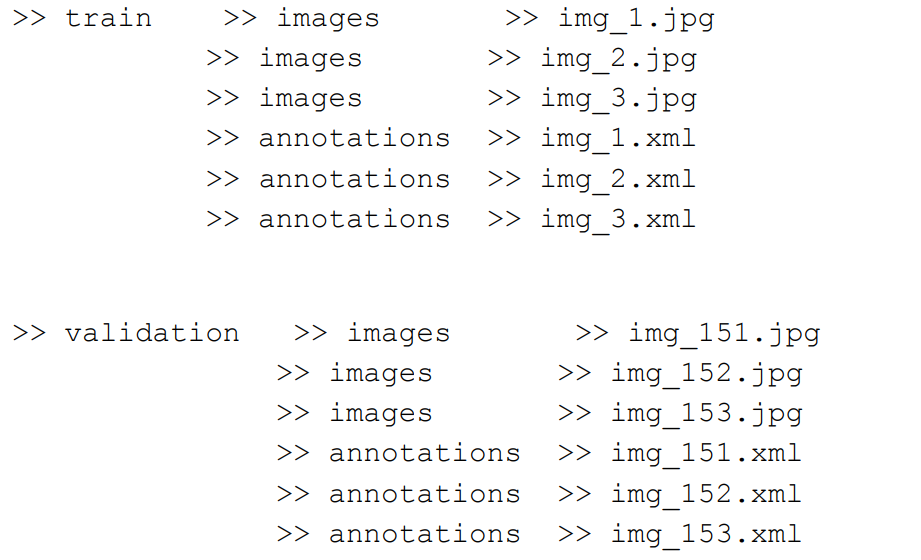
\includegraphics[width=0.5\linewidth]{figuras/MachineLearning/foldersDataset.png}
	\caption{Estrutura de pastas do \textit{dataset} de barcodes}
	\label{fig:foldersDataset}
\end{figure}

Ou seja, para cada imagem, há um arquivo XML com as anotações registradas pelo Labelimg. A etapa é o treinamento do modelo. Para tanto é necessário a compreensão da infraestrutura e bibliotecas utilizadas no projeto.

%------------------------------------------------

\subsection{Infraestrutura}

Com o intuito de acelerar o processo, foi utilizado um software online chamado Google Colaboratory que disponibiliza recursos de GPU para treinamento online. 

%------------------------------------------------

\subsubsection{Google Colaboratory}
O Google Colaboratory, mais conhecido como "Google Colab" ou simplesmente "Colab", é um projeto de pesquisa para criar protótipos de modelos de \textit{Machine Learning} em poderosas opções de \textit{hardware}, como GPUs e TPUs. Fornece um ambiente de notebook Jupyter sem servidor para desenvolvimento interativo. O Google Colab é gratuito para usar como outros produtos do G Suite, ferramenta corporativa do Google. \cite{colabdetail}
 
Características e Funcionalidades do Google Colab:

\begin{itemize}
    \item Suporte para Python 2.7 e Python 3.6;
    \item Aceleração de GPU;
    \item Bibliotecas pré-instaladas: diversas bibliotecas Python, como TensorFlow, Scikit-learn, Matplotlib etc.
    \item Recurso de colaboração: permite que os desenvolvedores usem e compartilhem o Jupyter notebook entre si sem precisar baixar, instalar ou executar qualquer coisa que não seja um navegador;
    \item Suporta comandos \textit{bash};
    \item Os notebooks do Google Colab são armazenados no drive.
\end{itemize}

\begin{figure}[H]
		\centering
		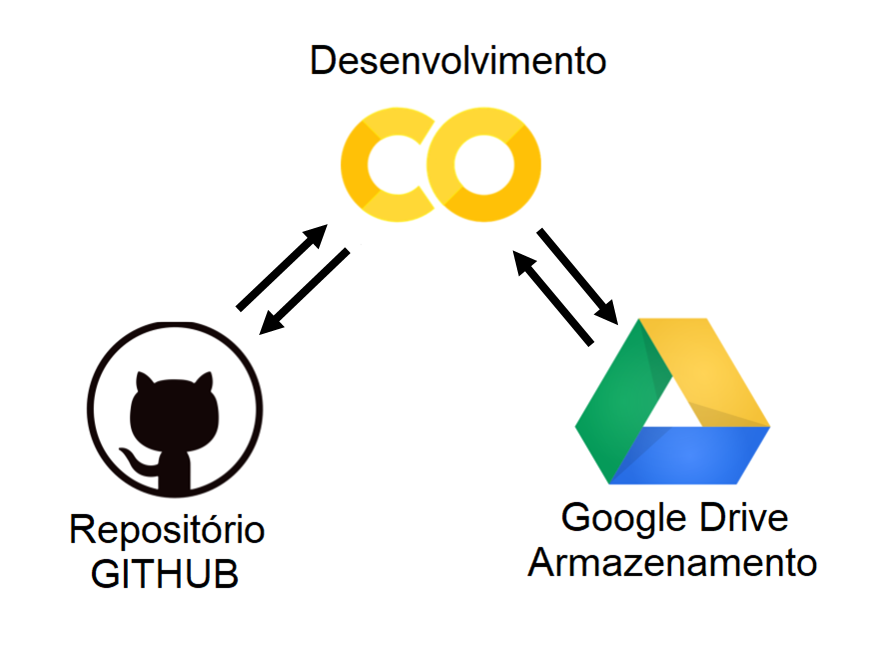
\includegraphics[scale=0.25]{figuras/MachineLearning/colabGithub.png}
		\caption{Utilização do Colab, Drive e Github}
		\label{fig:colabGithub}
\end{figure}

O Google Colab se integra facilmente ao Google Drive, fato que o torna uma opção direta como espaço de armazenamento dos dados e modelos. Porém há também outras opções de hospedagem de código, como por exemplo, a plataforma Github, escolhida para este trabalho.

\subsection{Blibliotecas utilizadas}

Todo o código foi implementado utilizando a linguagem de programação Python, e as seguintes bibliotecas foram utilizadas:

%------------------------------------------------p

\subsubsection{TensorFlow}

O TensorFlow é uma biblioteca Python de código aberto para implementar algoritmos de \textit{Machine Learning}. Um código utilizando o TensorFlow pode ser executado com pouca ou nenhuma alteração em uma ampla variedade de sistemas heterogêneos, desde dispositivos móveis, como telefones e tablets, até sistemas distribuídos em larga escala de centenas de máquinas e milhares de dispositivos computacionais, como placas de GPU.

O sistema é flexível e tem sido usado para conduzir pesquisas e implantar sistemas de \textit{Machine Learning} na produção de diversas áreas da ciência da computação e outros campos, incluindo reconhecimento de fala, visão computacional, robótica, recuperação de informações, processamento de idiomas, extração de informações geográficas e descoberta computacional de remédios. \cite{abadi2016tensorflow}

Vários serviços do Google utilizaram o TensorFlow em sua produção. O mesmo foi lançado como um projeto de código aberto e tornou-se amplamente utilizado para pesquisa de ML.\cite{199317}

%------------------------------------------------

\subsubsection{Scikit-Image}

O Scikit-image, também conhecido como Skimage, é uma biblioteca de processamento de imagens que implementa algoritmos e utilitários para uso em aplicações de pesquisa, educação e indústria. É lançado sob a licença liberal de código aberto Modified BSD, fornece uma API bem documentada na linguagem de programação Python e é desenvolvido por uma equipe internacional ativa de colaboradores.

O objetivo do scikit-image é fornecer uma biblioteca de alta qualidade de ferramentas e diversas de processamento de imagens, gratuitas e sem restrições. \cite{skimage}

%------------------------------------------------

\subsubsection{ImageAI}

ImageAI é uma biblioteca Python de código aberto desenvolvida para capacitar os desenvolvedores a criarem aplicativos e sistemas com recursos independentes de \textit{Deep Learning} e \textit{Computer Vision} usando poucas linhas de código.

A biblioteca ImageAI suporta previsão e treinamento de imagens usando 4 algoritmos diferentes de \textit{Machine Learning} treinados no conjunto de dados ImageNet-1000. O ImageAI também suporta detecção de objetos, detecção de vídeo e rastreamento de objetos usando RetinaNet, YOLOv3 e TinyYOLOv3 treinados no conjunto de dados COCO e PASCAL VOC.\cite{ImageAI}

Este trabalho utiliza a classe da biblioteca ImageAI chamada \textit{Custom Detection Model Training}, que possibilita o treinamento modelo próprio de detecção de objetos utilizando a arquitetura da YOLOv3.

%------------------------------------------------

\subsubsection{OpenCV}

O OpenCV (Open Source Computer Vision) é uma biblioteca de \textit{open source} e \textit{cross-plataform} (Multiplataforma) que contém mais de 500 algoritmos otimizados para análise de imagem e vídeo. \cite{opencv}

%------------------------------------------------

\subsection{Treinamento dos modelos}

Após gerado o conjunto de dados, é possível trabalhar no treinamento do modelo da rede neural. Para isso foi utilizado o \textit{framework} TensorFlow destinado à \textit{Deep Learning}. Além de uma rede neural pré-treinada chamada YoloV3, escrita em Python que faz uso das funções disponibilizadas pela biblioteca ImageAI .

Através do modelo da rede Yolov3, treina-se mais dois novos modelos de redes neurais:
\begin{itemize}
    \item Modelo de rede neural para reconhecimento de \textit{barcodes};
    \item Modelo de rede neural para reconhecimento de algarismos numéricos;
\end{itemize}

O resultado do treinamento são arquivos no formato .h5\footnote{Um arquivo h5 é um arquivo de dados salvo no formato \textit{Hierarchical Data Format}(HDF). Contém conjuntos multidimensionais de dados científicos.}. Cada arquivo é um modelo que é avaliado através da melhor acurácia, que indica uma performance geral do modelo. Dentre todas as classificações, quantas o modelo classificou corretamente.

%------------------------------------------------

\subsubsection*{YOLOv3}\label{sub:Yolov3}

A rede neural YOLOv3 evoluiu de YOLO e YOLO-V2 \cite{redmon2018yolov3}. Quando comparado com a rede Faster R-CNN, a mais eficiente das CNNs para detecção, a YOLO transforma o problema de detecção em um problema de regressão, em que a informação tem um significado numérico resultante de alguma previsão na imagem. Isto não requer uma região da proposta e gera coordenadas e probabilidades de bbox de cada classe diretamente por meio de regressão. Isso aumenta consideravelmente a velocidade de detecção em comparação com o Faster R-CNN.\cite{yolov3_apple}

O YOLO é a frequência mais rápida (45 FPS) do que outros algoritmos de detecção de objetos \cite{yolov3RealTime}.

O YOLO impõe fortes restrições espaciais nas previsões de bbox, pois cada célula da \textit{grid} prevê apenas duas \textit{box} e pode ter apenas uma classe. Essa restrição espacial limita o número de objetos próximos que o modelo pode prever. \cite{yolov3RealTime}

\begin{figure}[htbp]
		\centering
		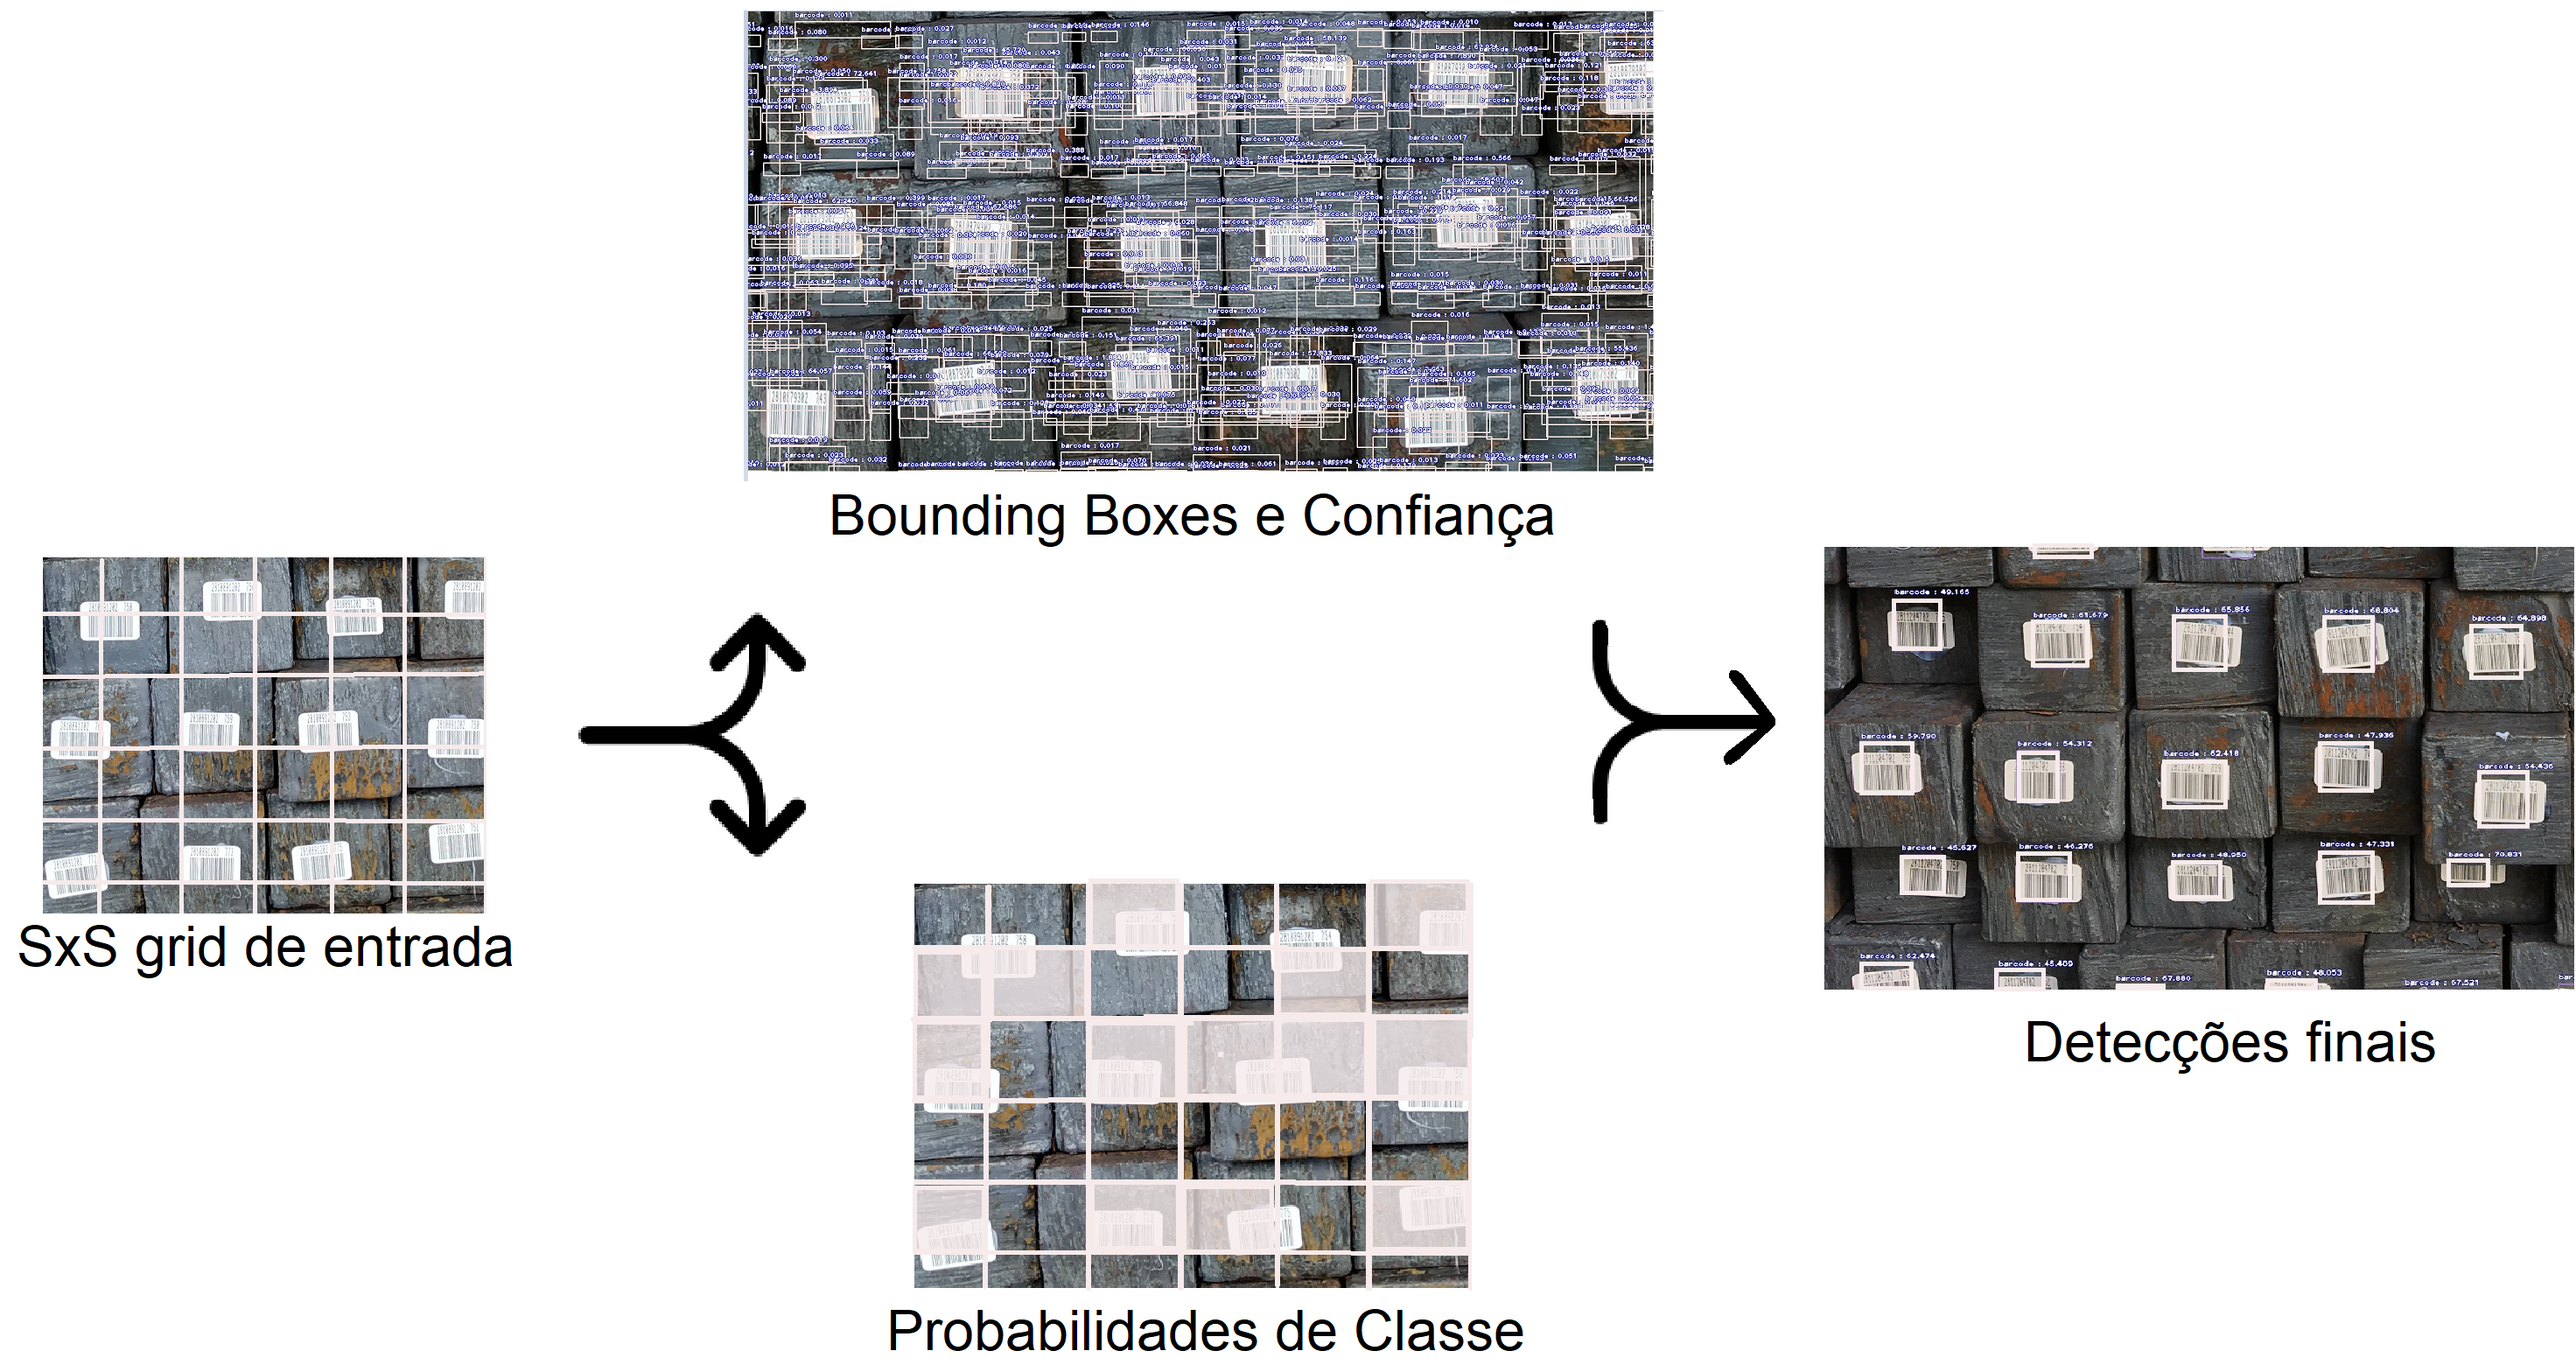
\includegraphics[scale=0.2]{figuras/MachineLearning/yolo.png}
		\caption{YOLO}
		\label{fig:yolo}
\end{figure}

No modelo de detecção YOLO (Figura \ref{fig:yolo}) uma única rede convolucional prediz tanto os bbox quanto as probabilidades de pertinência à classe de cada objeto detectado. Para isso, YOLO funciona da seguinte forma:

\begin{itemize}
    \item Toma-se uma imagem e divide-se-a em um grid SxS de células (S = 6);
    \item Usando o \textit{grid} como referência, gera-se N \textit{bounding boxes};
    \item \textit{Bounding boxes} com probabilidade acima de um limiar são selecionados e usados para localizar o objeto dentro da imagem.
\end{itemize}

Cada célula do  \textit{grid} é usada para predizer B bbox e C probabilidades de classe. O conceito de interseção sobre união (IoU) tem um papel importante e a confiança de uma predição em YOLO é dada por:

\begin{equation}
    Confianca = p_r(Object) X IoU_{pred}^{truth} , p_r(Object) \in \left \{ 1\right.,\left.0\right \}
\end{equation}

Quando o \textit{target} estiver no \textit{grid}, \(p_r(Object)\) = 1 e 0 caso contrário. \(IoU_{pred}^{truth}\) é usado para denotar a interseção sobre união e a previsão da bbox. 
A confiança reflete se o \textit{grid} contém objetos e a precisão da bbox prevista. Quando várias bbox detectam o mesmo \textit{target}, o YOLO usa o método de não supressão máxima (NMS) para selecionar a melhor bbox.

%------------------------------------------------

\section{Sistema Web} \label{sec:web}

Essa seção mostra as etapas necessárias de criação do sistema web desenvolvida para mostrar ao usuário final os resultados do sistema de detecção de objetos.

O sistema web foi criado para facilitar o gerenciamento, visualização e rastreabilidade das corridas para o operador através de um \textit{layout} amigável.

Nessa etapa foi utilizada a linguagem Node.JS para implementar o \textit{back-end} e as linguagens HTML, CSS,  e JavaScript para implementar o \textit{front-end}. 

Para a comunicação entre essas duas partes, foi utilizada a linguagem EJS que é uma linguagem de visualização, com ele é possível transportar dados do back-end para o front-end de maneira simples. Basicamente utiliza-se códigos em javascript no html das páginas. 

A escolha do Node.JS foi devido aos seguintes fatores:

\begin{itemize}
    \item instalação simples, não necessita de dependência para configuração;
    \item possibilidade de executar aplicações Node em qualquer plataforma;
    \item I/O não bloqueante. Ou seja, quando é necessário acessar um arquivo no disco, se comunicar com um \textit{Web Service} ou acessar um banco de dados, esse acesso é feito de forma assíncrona por padrão;
    \item ser escrito em JavaScript, o que simplifica o uso tecnologias \textit{front-end}, que na maioria, também são escritas em JavaScript.
\end{itemize}
 
%------------------------------------------------

\subsection{Node.JS}

O Node.JS, também conhecido como Node, é uma estrutura EDA\footnote{Modo de realizar a comunicação entre sistemas. Consiste, principalmente, em operações assíncronas, além de permitir aplicativos escalonáveis e gerar menor acoplamento entre os serviços, permitindo uma arquitetura flexível.} de código aberto para o desenvolvimento de aplicativos JavaScript em servidores. É baseado no \textit{runtime} do Google, chamado de motor V8. O V8 e o Node são implementados em C e C++, focados no desempenho e baixo consumo de memória. Embora o V8 suporte principalmente o uso de JavaScript no navegador, o Node foca no suporte de processos de servidores \cite{Tilkov2010}.

O Node é um dos \textit{frameworks} mais famosos que suportam o desenvolvimento de servidores utilizando o JavaScript \cite{Tilkov2010}.

%------------------------------------------------

\subsection{HTML}

Para disponibilizar informações para distribuição global, é preciso uma linguagem universalmente compreendida. A linguagem de publicação usada pela WWW\footnote{WWW é um sistema de documentos dispostos na Internet que permite o acesso às informações apresentadas no formato de hipertexto.} é HTML (da HyperText Markup Language).\citeauthor{html}

O HTML fornece aos autores os meios para: 
\begin{itemize}
    \item Publicar documentos \textit{online} com títulos, texto, tabelas, listas, fotos etc. 
    \item Recuperar informações \textit{online} por meio de links de hipertexto de maneira simples. 
    \item Criar formulários para realizar transações com serviços remotos, para busca de informações, reservas, pedidos de produtos etc. 
    \item Incluir planilhas, videoclipes, clipes de som e outros aplicativos diretamente em seus documentos.
\end{itemize}

%------------------------------------------------

\subsection{CSS}
Um dos padrões fundamentais do W3C \footnote{Trata-se de uma organização internacional responsável pelos protocolos e padronização da WWW, a rede mundial de computadores.} para o desenvolvimento de aplicativos da web é o \textit{Cascading Style Sheets}(CSS) \cite{Casca8378199:online,css}.

CSS é uma linguagem que define a semântica de apresentação dos elementos HTML, incluindo seu posicionamento, layout, cor e fontes. A principal vantagem da adoção do CSS é organização da estrutura de apresentação de maneira previsível . \cite{badros1999constraint}

%------------------------------------------------

% \subsection{Docker}

% Docker é um projeto \textit{open source} que foi inicialmente lançado em 2013, atraiu grande atenção na industria de TI. É uma plataforma de conteinerização que possibilita usuários a construir sua aplicação dentro de um conteiner e transferir conteiners através de máquinas com diferentes sistemas operacionais de um jeito simples. \cite{chang2017kubernetes}

% Existem três componentes principais do Docker:

% \begin{itemize}
% 	\item \textit{Docker images}: são \textit{templates} de leitura que servem como base para a criação de conteiners.;
% 	\item \textit{Docker registries}: é o local onde estão uma grande coleção de \textit{Docker images}.;
% 	\item \textit{Docker containers}: são as instâncias virtuais em que as aplicações estão rodando. Cada conteiner contem uma aplicação rodando e todas os seus arquivos de dependências, como o código, bibliotecas e utilitários do sistema.
% \end{itemize}

% A construção de imagens pode ser feita de duas maneiras. É possível criar um conteiner através de uma imagem já existente (\textit{docker run}), realizar modificações e instalações dentro do conteiner, parar o container e depois salvar o estado atual do conteiner como uma nova imagem (\textit{docker commit}). Este processo é parecido com uma instalação clássica de uma máquina virtual, mas deve ser feito para cada imagem caso haja alguma atualização, já que as imagens são padronizadas. Para automatizar o processo, \textit{Dockerfiles} nos permite especificar uma imagem de base e uma sequência de comandos que serão executados quando a imagem é construída, juntamente com outras opções de especificações, como portas a serem expostas. A imagem é depois construída com o comando \textit{docker build}.\cite{DiPietro}


%------------------------------------------------
\section{Arquitetura do projeto}

Ao fazer a escolha da arquitetura do projeto, optou-se por utilizar a arquitetura de \textit{microservices}, pois como haverá mais de um módulo de software com linguagens e características diferentes, torna-se mais fácil escalar e fazer manutenções de maneiras independentes.

\subsection{Microsserviços}
Seguindo a definição de \citeauthor{ms1} (\citeyear{ms1}), a arquitetura de microsserviços trata do desenvolvimento de uma aplicação que se baseia na existência de diversos pequenos serviços independentes. 

Os serviços podem comunicar-se utilizando mecanismos leves de interface, como HTTP. Porém, como cada serviço deve ser independente, uma alteração na implementação de um não deve afetar o funcionamento dos demais. \cite{Pahl}

Em suma os microsserviços são os resultados da decomposição funcional de uma aplicação. 

Um exemplo da arquitetura de microsserviços está na Figura \ref{fig:arquitetura-microsservicos}.

\begin{figure}[htbp]
	\centering
	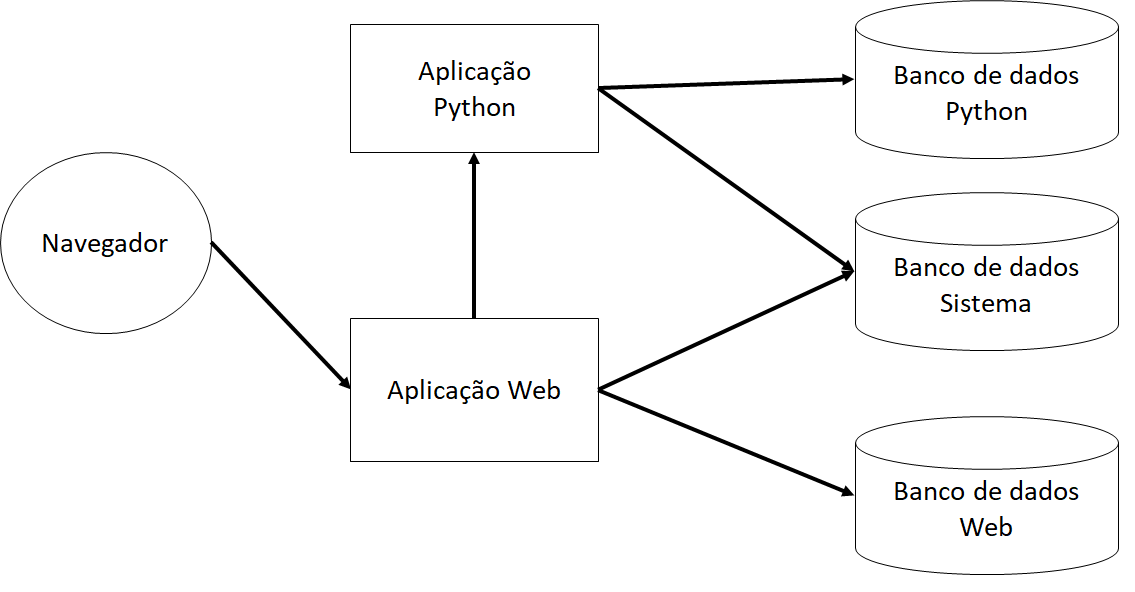
\includegraphics[width=1\linewidth]{figuras/WebService/microservices.png}
	\caption{Exemplo arquitetura de microsserviços.}
	\label{fig:arquitetura-microsservicos}
\end{figure}

 

%------------------------------------------------





